\chapter{Теоретическая часть}


\section{Современное состояние исследований в области сохранения цифрового культурного наследия}

Проблематика создания исторических информационных систем и формирования исследовательских инфраструктур представляет собой актуальное направление современной историографии, рассматриваемое как в теоретико-методологической, так и в практической плоскостях.
Центральным элементом данных исследований остается исторический источник, что соответствует фундаментальному подходу И.Д. Ковальченко, определившего задачу источниковедения в повышении информативной отдачи источников~\cite{1_kid2003}.
Развитие данной концепции привело к формированию качественно нового направления – «источниковедения 2.0», синтезирующего традиционные методы работы с историческими источниками и современные цифровые технологии~\cite{2_kornev2018}.

Теоретико-методологические дискуссии об исторических информационных системах развиваются в рамках нескольких взаимосвязанных направлений.
Профессиональное историческое сообщество активно исследует возможности применения цифровых технологий и инструментов к историческому источнику.
В российском научном пространстве ключевой площадкой для обсуждения данных вопросов является Ассоциация «История и компьютер», функционирующая с 1992 года и издающая специализированный журнал «Историческая информатика».
На страницах данного издания рассматриваются актуальные проблемы применения трехмерных реконструкций, технологий искусственного интеллекта и методов работы с большими данными в исторических исследованиях~\cite{3_belova1993}.
Существенную роль в институционализации цифровых методов в исторической науке играют специализированные центры Digital Humanities, созданные при Высшей школе экономики, Сибирском федеральном университете и ряде других ведущих образовательных учреждений~\cite{4_vladimirov2014}.

Образовательный потенциал исторических информационных систем анализируется исследователями в контексте подготовки специалистов для институтов памяти и формирования профессиональных компетенций историков~\cite{5_redkina2021}.
Особое внимание уделяется воспитательному эффекту проектов в области гражданской науки и цифровой публичной истории (digital public history)~\cite{6_barabucci2022}.
Интеграция цифровых методов в образовательный процесс рассматривается как необходимое условие формирования цифровых компетенций у будущих исследователей, способных эффективно работать в условиях цифровой трансформации гуманитарного знания.

Исторические информационные системы привлекают внимание специалистов в области управления информацией и работы с культурным наследием, включая библиотекарей, архивистов и музейных работников.
Задачи оцифровки исторических источников, успешно реализуемые с 1980-х годов, в современном контексте обсуждаются преимущественно с практической точки зрения: организация оцифрованных коллекций, выбор программного обеспечения, реализация поисковых механизмов~\cite{7_yumashova2016}.
В рамках данного направления поднимаются фундаментальные вопросы цифровой трансформации институтов памяти и обеспечения долговременной сохранности цифрового культурного наследия.

Проблема сохранности цифрового культурного наследия приобретает критическую важность в условиях стремительного развития информационных технологий и постоянной эволюции форматов данных.
В Российской Федерации отсутствует комплексная государственная политика сохранения цифрового культурного наследия, закрепленная на законодательном уровне.
Существующие инициативы носят фрагментарный характер и представлены отдельными исследовательскими и общественными проектами~\cite{8_gorlova2021}.
Среди наиболее значимых следует отметить деятельность АНО «Информационная культура», осуществляющей систематическую архивацию российского сегмента интернета.

Современные исследователи работают с теми же объектами изучения, которые ученые исследовали на протяжении столетий, достигнув глубокого понимания информации традиционными методами.
Однако создаваемые цифровые инструменты позволяют систематизировать, верифицировать и переосмыслить существующие историографические концепции, а также формулировать новые теоретические построения, возникающие при абстрагировании от частных деталей исследуемого материала.

Круг обсуждаемых вопросов относительно исторических информационных систем характеризуется значительной широтой и междисциплинарностью.
Однако отсутствие полноценных исследовательских инфраструктур в понимании digital humanities препятствует комплексному решению теоретических и прикладных задач.
Необходимо выстраивание вокруг исторического источника как набора данных интегрированной системы, включающей информационные стратегии пользователей, техническую и технологическую инфраструктуру, а также методическую поддержку исследовательской деятельности.

Данный проект направлен на разработку научно обоснованной модели исторической информационной системы, базирующейся на материалах по истории Сибири.
Результатом работы должна стать концептуальная основа для создания национальной информационной инфраструктуры в области гуманитарных наук.


\section{Проектирование архитектуры серверной части}

\subsection{Выбор технологий и инструментов}

Процесс выбора технологий и инструментов представляет собой критический этап проектирования программного обеспечения, оказывающий определяющее влияние на успешность реализации проекта.
Оптимальный технологический стек непосредственно воздействует на качественные характеристики, эффективность и экономические параметры процесса разработки.
Необходимо учитывать комплекс факторов, включающих функциональные и нефункциональные требования проекта, компетенции команды разработчиков, потенциал масштабируемости, вопросы совместимости и долгосрочной поддержки. Анализ современных технологий и инструментов, применяемых в разработке программного обеспечения, их преимуществ и ограничений позволяет принимать обоснованные архитектурные решения для конкретного проекта.


Проведенный анализ современных технологий в сфере разработки backend-приложений выявил следующие ключевые платформы.
Python представляет собой высокоуровневый язык программирования общего назначения с динамической строгой типизацией и автоматическим управлением памятью~\cite{9_rana2019}, ориентированный на повышение производительности разработчика, читаемости кода и обеспечение переносимости программ~\cite{10_sirunyan2020}. Основными ограничениями Python являются относительно низкая производительность интерпретируемого кода и особенности работы с многопоточностью, обусловленные механизмом Global Interpreter Lock (GIL).

Ruby характеризуется как динамический, рефлективный, интерпретируемый высокоуровневый язык программирования~\cite{11_roganov2008}. Данная платформа демонстрирует определенные сложности с реализацией многопоточных вычислений, что может негативно влиять на производительность приложений. Несмотря на значительную популярность языка, формирование активного сообщества разработчиков происходит постепенно.

PHP, получивший наибольшее распространение благодаря широкой поддержке на хостинг-платформах и веб-серверах, демонстрирует оптимальные характеристики для небольших систем. Однако данная технология обладает существенными ограничениями при создании масштабируемых решений корпоративного уровня.

Java представляет собой строго типизированный объектно-ориентированный язык программирования общего назначения.
Приложения Java компилируются в специальный байт-код, обеспечивающий возможность выполнения на любой компьютерной архитектуре с реализацией виртуальной Java-машины~\cite{12_schildt2019}. Данная технология обеспечивает высокую производительность, надежность и кроссплатформенность, что делает ее предпочтительным выбором для enterprise-решений.

Go, разработанный компанией Google, предназначен для создания высокопроизводительных приложений с поддержкой масштабирования и параллельного выполнения. Язык отличается высокой скоростью выполнения и естественной адаптивностью к микросервисной архитектуре, что обусловлено встроенными механизмами конкурентного программирования.

Для реализации данного проекта в качестве основной технологической платформы выбран язык Java, обладающий комплексом преимуществ: высокой скоростью выполнения, производительностью и кроссплатформенностью.
Spring Framework, являющийся де-факто стандартом для enterprise-разработки на Java, позволяет создавать сложные и масштабируемые приложения благодаря архитектуре, основанной на принципах инверсии управления и внедрения зависимостей. Данные архитектурные принципы обеспечивают создание модульного, слабосвязанного и легко расширяемого кода, способного эффективно масштабироваться в соответствии с растущими требованиями.

Фундаментальными преимуществами использования Java и Spring являются их надежность и встроенные механизмы безопасности.
Java обеспечивает безопасность посредством механизма виртуальной машины, позволяющего выполнять код в изолированном окружении.
Spring предоставляет комплексные инструменты для защиты приложений от известных уязвимостей, включая межсайтовый скриптинг (XSS) и подделку межсайтовых запросов (CSRF). Дополнительным преимуществом является наличие обширного сообщества разработчиков, обеспечивающего доступность документации, примеров кода и оперативной поддержки.

Полный технологический стек проекта включает следующие компоненты: Spring Cloud Config для централизованного управления конфигурациями, Eureka Service Discovery для обнаружения сервисов, Spring Cloud Gateway в качестве API-шлюза, Spring Cloud Circuit Breaker и Resilience4j для обеспечения отказоустойчивости, Spring Cloud Sleuth для распределенной трассировки, Spring Cloud Stream и Spring Kafka для асинхронного обмена сообщениями, Kafka Streams API для потоковой обработки данных, Keycloak для управления идентификацией и доступом, а также React и Redux для построения пользовательского интерфейса.

Spring Cloud Config представляет собой инструмент, обеспечивающий централизованное хранение конфигурации приложений и их динамическое обновление без перезапуска.
Данное решение позволяет хранить конфигурации микросервисов на удаленном сервере и получать эти настройки во время запуска приложения. Это существенно упрощает управление конфигурацией в системах с множеством микросервисов и при реализации практик непрерывной интеграции и развертывания~\cite{13_davis2020}.
Spring Cloud Config обеспечивает шифрование конфиденциальных данных перед сохранением на удаленном сервере, что гарантирует конфиденциальность критически важной информации и обеспечивает дополнительный уровень безопасности приложения.

Spring Cloud API Gateway представляет собой отдельное Spring Boot приложение, реализующее паттерн обратного прокси-сервера.
Все запросы проходят через данный компонент, который выполняет функции маршрутизации и фильтрации.
Микросервисы не взаимодействуют напрямую, а обращаются к прокси-серверу, который также является единственной точкой входа для внешних пользователей. Прокси-сервер анализирует входящий запрос, определяет целевой микросервис, перенаправляет запрос и возвращает ответ клиенту.

Схема работы представлена на рисунке~\ref{fig:api_gateway}.

\begin{figure}[htbp]
    \centering
    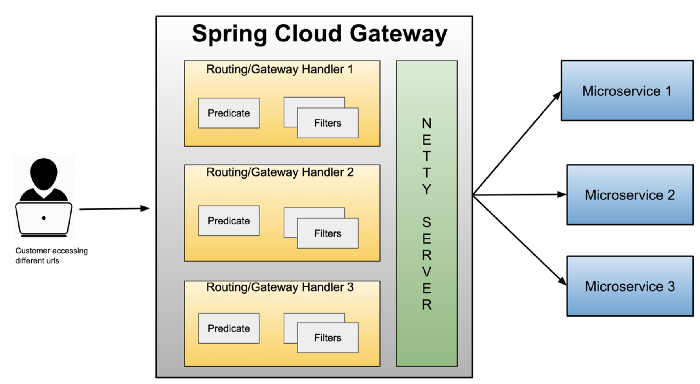
\includegraphics[width=0.8\textwidth]{Dissertation/images/api_gateway}
    \caption{Диаграмма работы API Gateway}
    \label{fig:api_gateway}
\end{figure}

Spring Cloud Circuit Breaker представляет собой библиотеку, предоставляющую абстракцию для реализации паттерна Circuit Breaker в микросервисных приложениях.
Данный паттерн используется для управления ошибками и сбоями в распределенных системах. Механизм позволяет ограничивать количество обращений к недоступным или нестабильным сервисам, перенаправляя запросы на резервные сервисы или возвращая предопределенные значения для предотвращения каскадных сбоев и минимизации времени простоя системы.

Spring Cloud Circuit Breaker поддерживает различные реализации паттерна, включая Hystrix и Resilience4j, причем в данном проекте используется последний. Библиотека предоставляет унифицированный интерфейс для вызова удаленных сервисов через Circuit Breaker, а также обеспечивает интеграцию со Spring Cloud Discovery для автоматического обнаружения и регистрации сервисов в среде выполнения.

Eureka Service Discovery представляет собой библиотеку, реализующую механизм обнаружения и регистрации сервисов в распределенной системе. Данное решение критически важно в микросервисной архитектуре, где каждый сервис может быть развернут на различных узлах и портах, а клиентам необходима актуальная информация об адресах для доступа к сервисам.

Eureka обеспечивает возможность сервисам регистрироваться в централизованном реестре и получать информацию об адресах других сервисов.
Клиенты используют Eureka для поиска и обращения к необходимым сервисам по их логическим именам без необходимости хранения жестко закодированных адресов. Система предоставляет дополнительные функции мониторинга состояния сервисов и отслеживания изменений их конфигурации. При возникновении сбоев или перезапусках сервисов Eureka автоматически обновляет информацию в реестре, что обеспечивает устойчивость к отказам и минимизацию времени недоступности~\cite{13_davis2020}.

Разработчики могут использовать библиотеку Spring Cloud Netflix Eureka для интеграции Service Discovery в приложения на Spring.
Библиотека предоставляет декларативный подход через аннотации и конфигурационные классы для регистрации сервисов и обращения к ним через реестр Eureka.

Keycloak представляет собой комплексное решение для управления идентификацией и доступом с открытым исходным кодом.
Система предоставляет функциональность единого входа, аутентификации, авторизации, социального входа и федерации пользователей.
Keycloak поддерживает множество протоколов аутентификации, включая OAuth2, OpenID Connect, SAML и Kerberos, что обеспечивает гибкость и возможность адаптации к требованиям различных предметных областей. Административная веб-консоль Keycloak предоставляет удобный интерфейс для управления пользователями, ролями, разрешениями и клиентскими приложениями.

Apache Kafka представляет собой распределенную платформу потоковой передачи данных с открытым исходным кодом, разрабатываемую Apache Software Foundation на языках Java и Scala.
Kafka функционирует как брокер сообщений, сохраняющий данные от процессов-производителей в формате «ключ-значение».
Данные организуются в разделы в рамках различных тем~\cite{14_niya2019}. Внутри каждого раздела сообщения строго упорядочены по смещениям, определяющим позицию сообщения, и индексируются с сохранением временных меток.
Процессы-потребители осуществляют чтение сообщений из разделов.
Для потоковой обработки Kafka предоставляет Streams API, позволяющий разрабатывать Java-приложения для обработки потоков данных.

Схема работы представлена на рисунке~\ref{fig:kafka_architecture}.
\begin{figure}[htbp]
    \centering
    % Placeholder для диаграммы архитектуры Apache Kafka
    
\includegraphics[width=0.7\textwidth]{Dissertation/images/kafka_scheme}
    \caption{Архитектура Apache Kafka}
    \label{fig:kafka_architecture}
\end{figure}

\subsection{Проектирование структуры приложения}

После определения современного технологического стека необходимо спроектировать архитектуру продукта для формирования стратегии развития и устранения потенциальных противоречий на этапе проектирования.

В основу архитектурного решения положен подход микросервисной архитектуры, который в сравнении со стандартным монолитным RESTful API обладает рядом существенных преимуществ.
Гибкость микросервисной архитектуры проявляется в возможности независимого добавления, удаления или модификации отдельных сервисов без влияния на функционирование остальной системы. Данная характеристика критически важна для проекта, предполагающего распределенную разработку несколькими группами из различных географических локаций, обеспечивая эффективное делегирование обязанностей.

Масштабируемость реализуется через возможность независимого масштабирования каждого микросервиса, что позволяет оперативно реагировать на изменение нагрузки. Учитывая неравномерное использование различных сервисов в разные временные периоды, данный подход обеспечивает оптимальное использование вычислительных ресурсов~\cite{15_dragoni2017}.

Удобство командной разработки обеспечивается возможностью независимой разработки, тестирования и развертывания каждого микросервиса. Принимая во внимание планируемую интеграцию со сторонними сервисами для расширения технологической среды исторических исследований, данное преимущество приобретает особую актуальность.

Высокая доступность достигается через размещение микросервисов в специализированных кластерах с поддержкой репликации и оркестрации. Механизмы автоматического восстановления отдельных сервисов в случае их отказа обеспечивают устойчивость системы к сбоям~\cite{16_schermann2016}.

На основании проведенного анализа была разработана архитектурная схема проекта, отражающая основные компоненты и их взаимосвязи, она представлена на рисунке~\ref{fig:microservices_schema}.

\begin{figure}[htbp]
    \centering
    % Placeholder для схемы микросервисной архитектуры проекта
    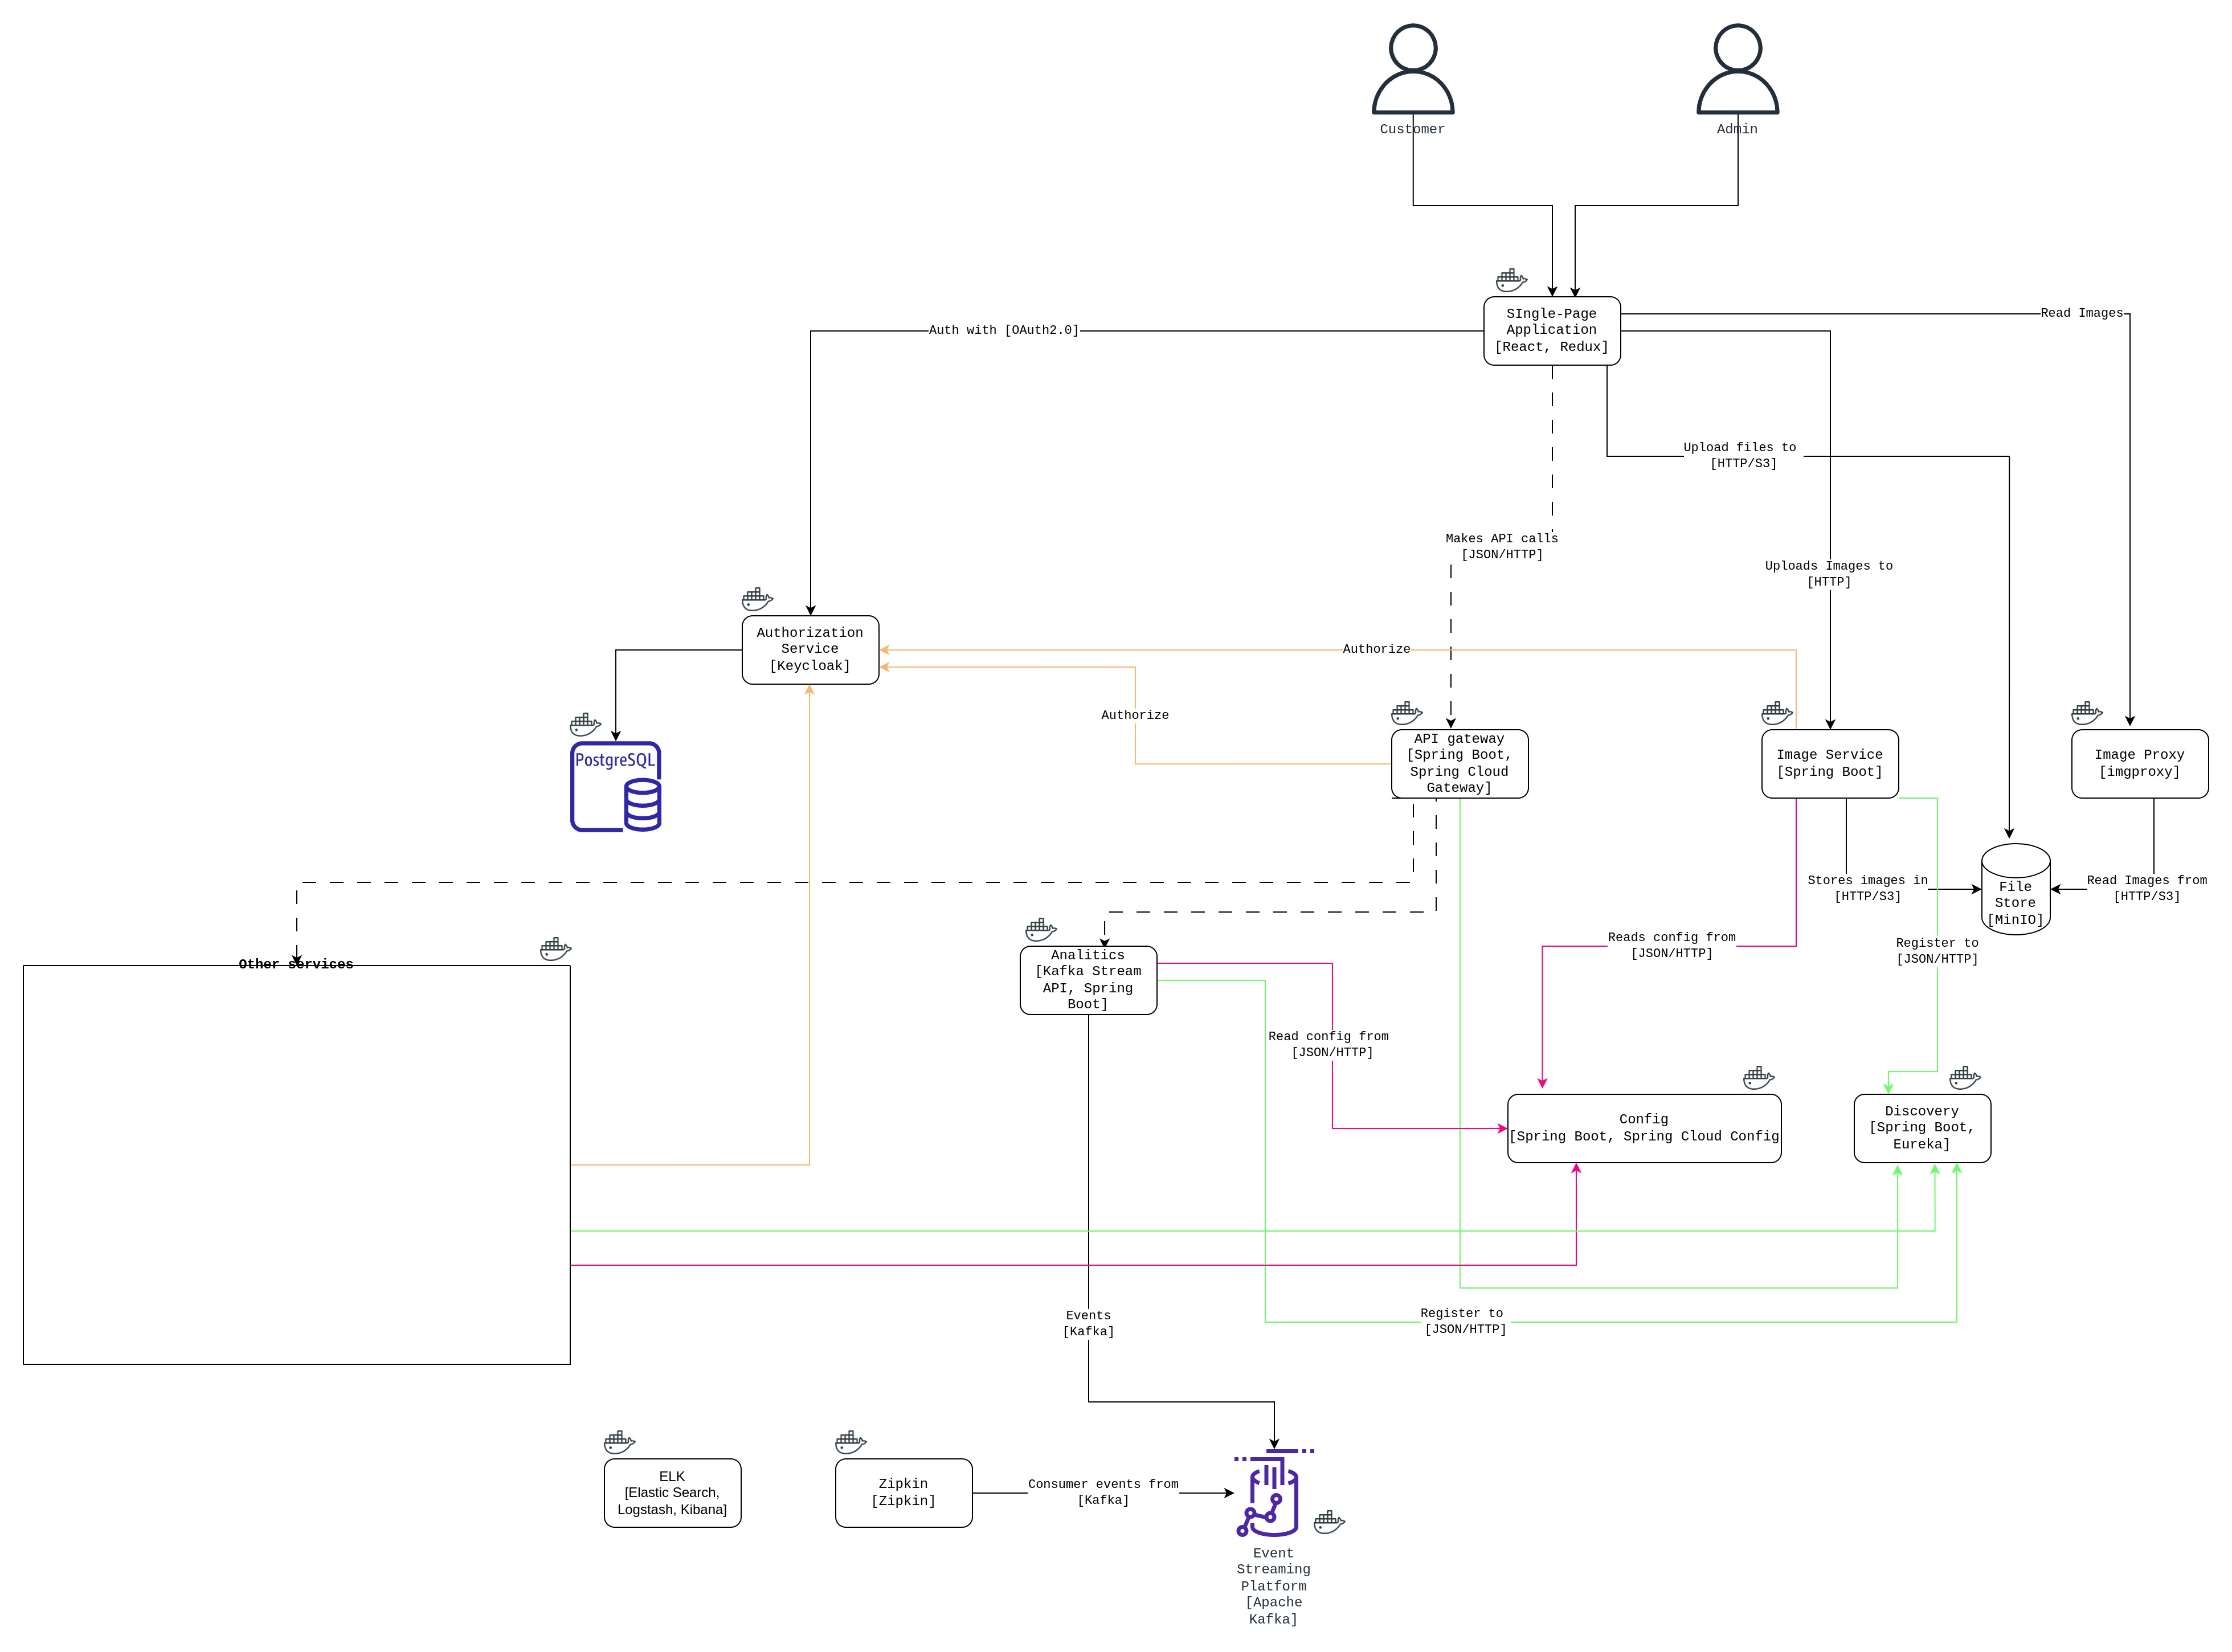
\includegraphics[width=0.7\textwidth]{Dissertation/images/project_scheme}
    \caption{Схема микросервисной архитектуры проекта}
    \label{fig:microservices_schema}
\end{figure}

Внедрение сервера конфигурации в инфраструктуру микросервисов обладает критической важностью для обеспечения стабильности, управляемости и масштабируемости распределенных систем. Данный компонент представляет собой централизованное решение для управления конфигурационными параметрами, обеспечивающее консистентность и согласованность между различными компонентами системы.

Централизованное управление настройками множества микросервисов решает проблему консистентности конфигураций в условиях, когда каждый микросервис обладает уникальными параметрами. Это особенно критично в распределенных системах, где конфигурационные изменения должны оперативно и синхронно применяться ко всем компонентам инфраструктуры.

Централизованное хранение конфигураций существенно упрощает процессы обновления и развертывания микросервисов.
Возможность динамического изменения параметров конфигурации без перезапуска микросервисов сокращает время простоя системы. Данная характеристика является критически важной для бизнес-критичных приложений, требующих высокой доступности.

Сервер конфигурации существенно улучшает безопасность системы через централизованное управление конфиденциальными данными.
Ключи API и пароли хранятся в зашифрованном виде и предоставляются исключительно авторизованным микросервисам. Данный подход минимизирует риски утечек данных и упрощает управление доступом к чувствительной информации.

Улучшение масштабируемости достигается через эффективное управление конфигурациями при росте количества микросервисов. Сервер конфигурации обеспечивает быстрый и гибкий доступ к необходимым параметрам независимо от масштаба системы.

\paragraph{Критерии выбора сервера конфигурации}

При выборе сервера конфигурации для платформы анализа исторических данных необходимо учитывать комплекс критериев, обеспечивающих надежную и эффективную работу инфраструктуры.
Первостепенным требованием является обеспечение высокой доступности через механизмы автоматического восстановления и горизонтального масштабирования. Критически важными факторами являются минимизация задержек при доступе к конфигурационным файлам и поддержка различных форматов данных, включая JSON и YAML.

Лицензионные условия использования требуют тщательного анализа. Необходимо детальное изучение условий лицензирования и возможностей использования в коммерческих и некоммерческих проектах.
Обязательным требованием является поддержка шифрования конфигураций как в состоянии покоя, так и при передаче данных. Наличие активного сообщества разработчиков, хотя и является опциональным требованием, существенно влияет на долгосрочную поддержку и развитие продукта.

\paragraph{Сравнительный анализ решений для управления конфигурациями}

Для обоснованного выбора решения проведен сравнительный анализ трех наиболее распространенных инструментов управления конфигурациями в распределенных системах: Consul, etcd и Spring Cloud Config. Каждое из данных решений обладает уникальными характеристиками, определяющими область их оптимального применения.

Consul, разработанный компанией HashiCorp, представляет собой комплексную распределенную систему, объединяющую функции управления конфигурациями, обнаружения сервисов и организации сервисной сети. Consul предоставляет интегрированную функциональность для регистрации сервисов, мониторинга их состояния, распределенного хранения конфигураций и автоматизации сетевого взаимодействия.

Преимущества Consul включают автоматическое обнаружение и регистрацию сервисов, встроенные механизмы проверки состояния, использование распределенного KV-хранилища и поддержку функций сервисной сети с управлением сетевыми политиками. Однако сложность настройки и интеграции, особенно в крупных кластерах, а также высокие требования к ресурсам могут ограничивать применение в небольших проектах.

etcd, разработанный CoreOS, представляет собой распределенное хранилище конфигураций, основанное на алгоритме консенсуса Raft. Данное решение широко используется в экосистеме Kubernetes для хранения конфигурационных данных и метаданных.
etcd обеспечивает строгое согласование данных, высокую производительность, низкую задержку доступа и простое API. Глубокая интеграция с Kubernetes делает его естественным выбором для контейнеризованных приложений. Ограничения включают отсутствие встроенных механизмов обнаружения сервисов и сложность управления кластером в больших масштабах.

Spring Cloud Config представляет собой специализированный инструмент для управления конфигурациями в облачных приложениях экосистемы Spring. Решение обеспечивает централизованное управление конфигурационными файлами с поддержкой динамических изменений.
Глубокая интеграция с экосистемой Spring, централизованное управление и поддержка версионирования через системы контроля версий являются ключевыми преимуществами. Ограничения включают узкую специализацию на управлении конфигурациями и оптимизацию исключительно для Spring-приложений.

\paragraph{Реализация Configuration Service}

Configuration Service обеспечивает поддержку управления внешними конфигурациями в распределенной системе. Хранилище конфигураций версионируется под контролем Git и поддерживает изменения во время выполнения.
Сервер предоставляет REST API для получения конфигураций микросервисами.

Конфигурационные файлы в текущей реализации размещаются в classpath.
Сервер поддерживает шифрование и расшифровку значений свойств. По умолчанию используется симметричная криптография, а при запуске с профилем <<docker>> применяется асимметричная криптография.

Поддержка шифрования позволяет использовать публичные репозитории для хранения конфиденциальных данных.
Зашифрованные значения маркируются префиксом \texttt{\{cipher\}}. Для симметричной криптографии необходима установка свойства \texttt{encrypt.key}.
Асимметричная криптография требует настройки хранилища ключей через утилиту Java keytool:

\begin{lstlisting}
keytool -genkeypair -alias configkey -keyalg RSA
-dname "CN=Web Server,C=RU,S=OH" -keypass cfg-password
-keystore keystore.jks -storepass secure-keystore-password
\end{lstlisting}

\paragraph{Заключение по выбору сервера конфигурации}

Выбор инструмента для управления конфигурациями определяется спецификой проекта и архитектурными требованиями. Consul оптимален для комплексных систем с требованиями управления сетевой политикой. etcd представляет лучший выбор для высокопроизводительного хранения данных в Kubernetes-окружении. Spring Cloud Config является идеальным решением для централизованного управления конфигурациями в Spring-приложениях, что обосновывает его выбор для данного проекта.


В качестве реестра сервисов используется Netflix Eureka, предоставляющая REST API для регистрации и обнаружения сервисов.
Реестр служб обеспечивает балансировку нагрузки на стороне клиента и отделяет поставщиков услуг от потребителей без использования DNS.

Каждая служба регистрируется в реестре и периодически отправляет сигналы жизнедеятельности для подтверждения доступности. Механизм heartbeat обеспечивает актуальность информации о состоянии сервисов в реестре.
Клиенты запрашивают реестр для получения списка доступных экземпляров службы.

После получения списка доступных экземпляров клиент применяет алгоритм балансировки нагрузки для выбора целевого экземпляра. Локальное кеширование регистраций Eureka на стороне клиента минимизирует количество обращений к реестру и повышает производительность системы.

В контексте современных цифровых экосистем API Gateway представляет собой критически важное архитектурное решение, обеспечивающее рационализацию и организацию потока данных между клиентами и целевыми микросервисами.
Данный компонент предоставляет комплексную функциональность маршрутизации, фильтрации и авторизации трафика. API Gateway является одним из ключевых элементов микросервисной архитектуры, обеспечивающим организацию как внутренних, так и внешних взаимодействий между компонентами системы.


В определенных архитектурных сценариях рассматривается возможность прямого взаимодействия клиента с микросервисами.
Данный подход предполагает непосредственную отправку запросов клиентским приложением к отдельным микросервисам без промежуточных компонентов.
Каждый микросервис предоставляет общедоступный эндпоинт с индивидуальным TCP-портом для обеспечения прямого доступа.

Такой подход отражен на рисунке~\ref{fig:direct_client_service}.
\begin{figure}[htbp]
    \centering
    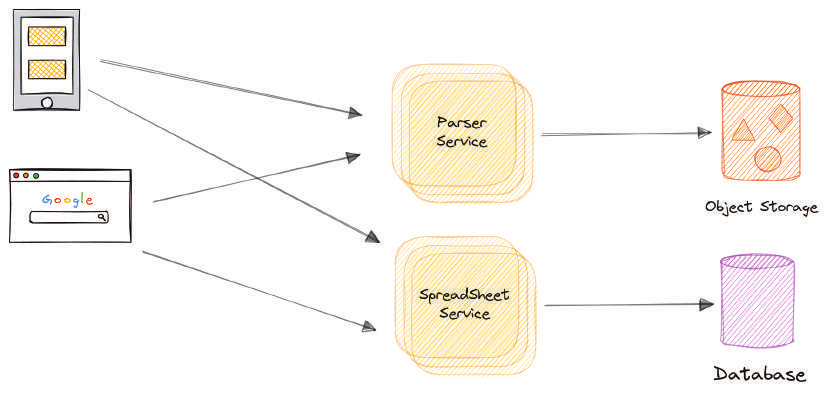
\includegraphics[width=0.7\textwidth]{Dissertation/images/wo_gateway}
    \caption{Схема прямого взаимодействия клиента и микросервиса}
    \label{fig:direct_client_service}
\end{figure}

При прямом взаимодействии возникает необходимость в механизмах управления трафиком и обеспечения безопасности~\cite{trebichavsky2021}. В данном контексте могут применяться балансировщики нагрузки или контроллеры доставки приложений, обеспечивающие равномерное распределение запросов и базовый уровень защиты через SSL-шифрование.

Однако при создании масштабных микросервисных приложений, особенно при взаимодействии с мобильными приложениями или одностраничными веб-приложениями, возникает комплекс критических проблем~\cite{microsoft_api_gateway}. Масштабирование системы требует минимизации обращений к серверной части, управления сквозными задачами авторизации и безопасности, создания специализированных фасадов для различных типов клиентов~\cite{newman2015building}.

Прямое соединение клиента с сервисами приводит к нелинейному увеличению сложности взаимодействия. Необходимость поддержания соединения на протяжении всего запроса существенно увеличивает нагрузку на сетевые ресурсы.
Отсутствие централизованного механизма контроля аутентификации создает серьезные проблемы безопасности. Поддержание единой политики безопасности становится практически невозможным из-за необходимости реализации собственной системы безопасности в каждом сервисе.

Прямое взаимодействие существенно усложняет процессы обновления и масштабирования.
Внесение изменений в микросервисы требует обновления всех клиентских приложений, что представляет собой трудоемкий и времязатратный процесс.


Шаблон API Gateway представляет собой архитектурную концепцию для масштабных микросервисных приложений с множественными клиентскими интерфейсами.
API Gateway функционирует как централизованная точка входа для определенных кластеров микросервисов. Данный паттерн, аналогичный концепции фасада в объектно-ориентированном проектировании, является фундаментальным элементом децентрализованных систем.

API Gateway, размещенный между клиентскими приложениями и микросервисами, функционирует как обратный прокси-сервер, маршрутизирующий запросы к соответствующим сервисам~\cite{zhao2018management}. Помимо маршрутизации, API Gateway обеспечивает комплексную функциональность, включающую аутентификацию, SSL-терминацию и кэширование.

Примерная схема изображена на рисунке~\ref{fig:api_gateway_interaction}
\begin{figure}[htbp]
    \centering
    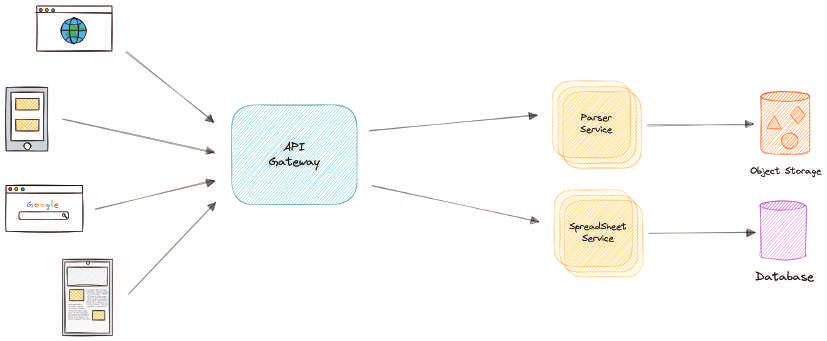
\includegraphics[width=0.7\textwidth]{Dissertation/images/gateway_project_scheme}
    \caption{Схема взаимодействия клиентов с микросервисами через API Gateway}
    \label{fig:api_gateway_interaction}
\end{figure}

Использование единого API Gateway для обслуживания различных клиентских приложений может создавать риски в плане масштабирования и поддержки. Разнообразие требований клиентских приложений может привести к превращению API Gateway в монолитный сервис.
Рекомендуется разделение API Gateway на несколько служб в соответствии с бизнес-границами и потребностями клиентов.


Разделение уровня API Gateway на несколько компонентов основывается на создании специализированных эндпоинтов для различных типов клиентов(рис~\ref{fig:bff_pattern}). Паттерн Backend for Frontend предполагает предоставление API Gateway специализированного интерфейса для конкретного типа клиентского приложения~\cite{alkhodary2023evaluation}.

\begin{figure}[htbp]
    \centering
    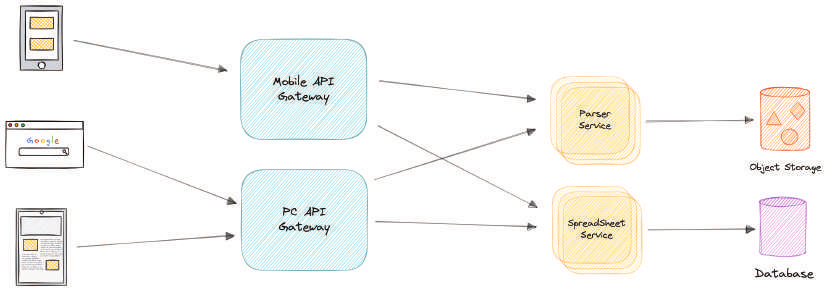
\includegraphics[width=0.7\textwidth]{Dissertation/images/bff}
    \caption{Архитектурный паттерн Backend for Frontend (BFF)}
    \label{fig:bff_pattern}
\end{figure}

Для платформ с множеством сервисов применение агрегации становится критически важным для объединения низкоуровневых вызовов~\cite{newman2015building}.
Один вызов к BFF-шлюзу порождает серию низкоуровневых обращений к различным микросервисам. В контексте платформы аналитики исторических данных это может включать получение координат церквей из определенного уезда для визуализации перемещения рукописей.

Оптимизация ресурсов достигается через максимальную параллелизацию вызовов. После завершения начального вызова к сервису поиска координат последующие обращения к другим сервисам выполняются параллельно для минимизации общего времени обработки(рис.~\ref{fig:bff_parallel_processing}).

\begin{figure}[htbp]
    \centering
    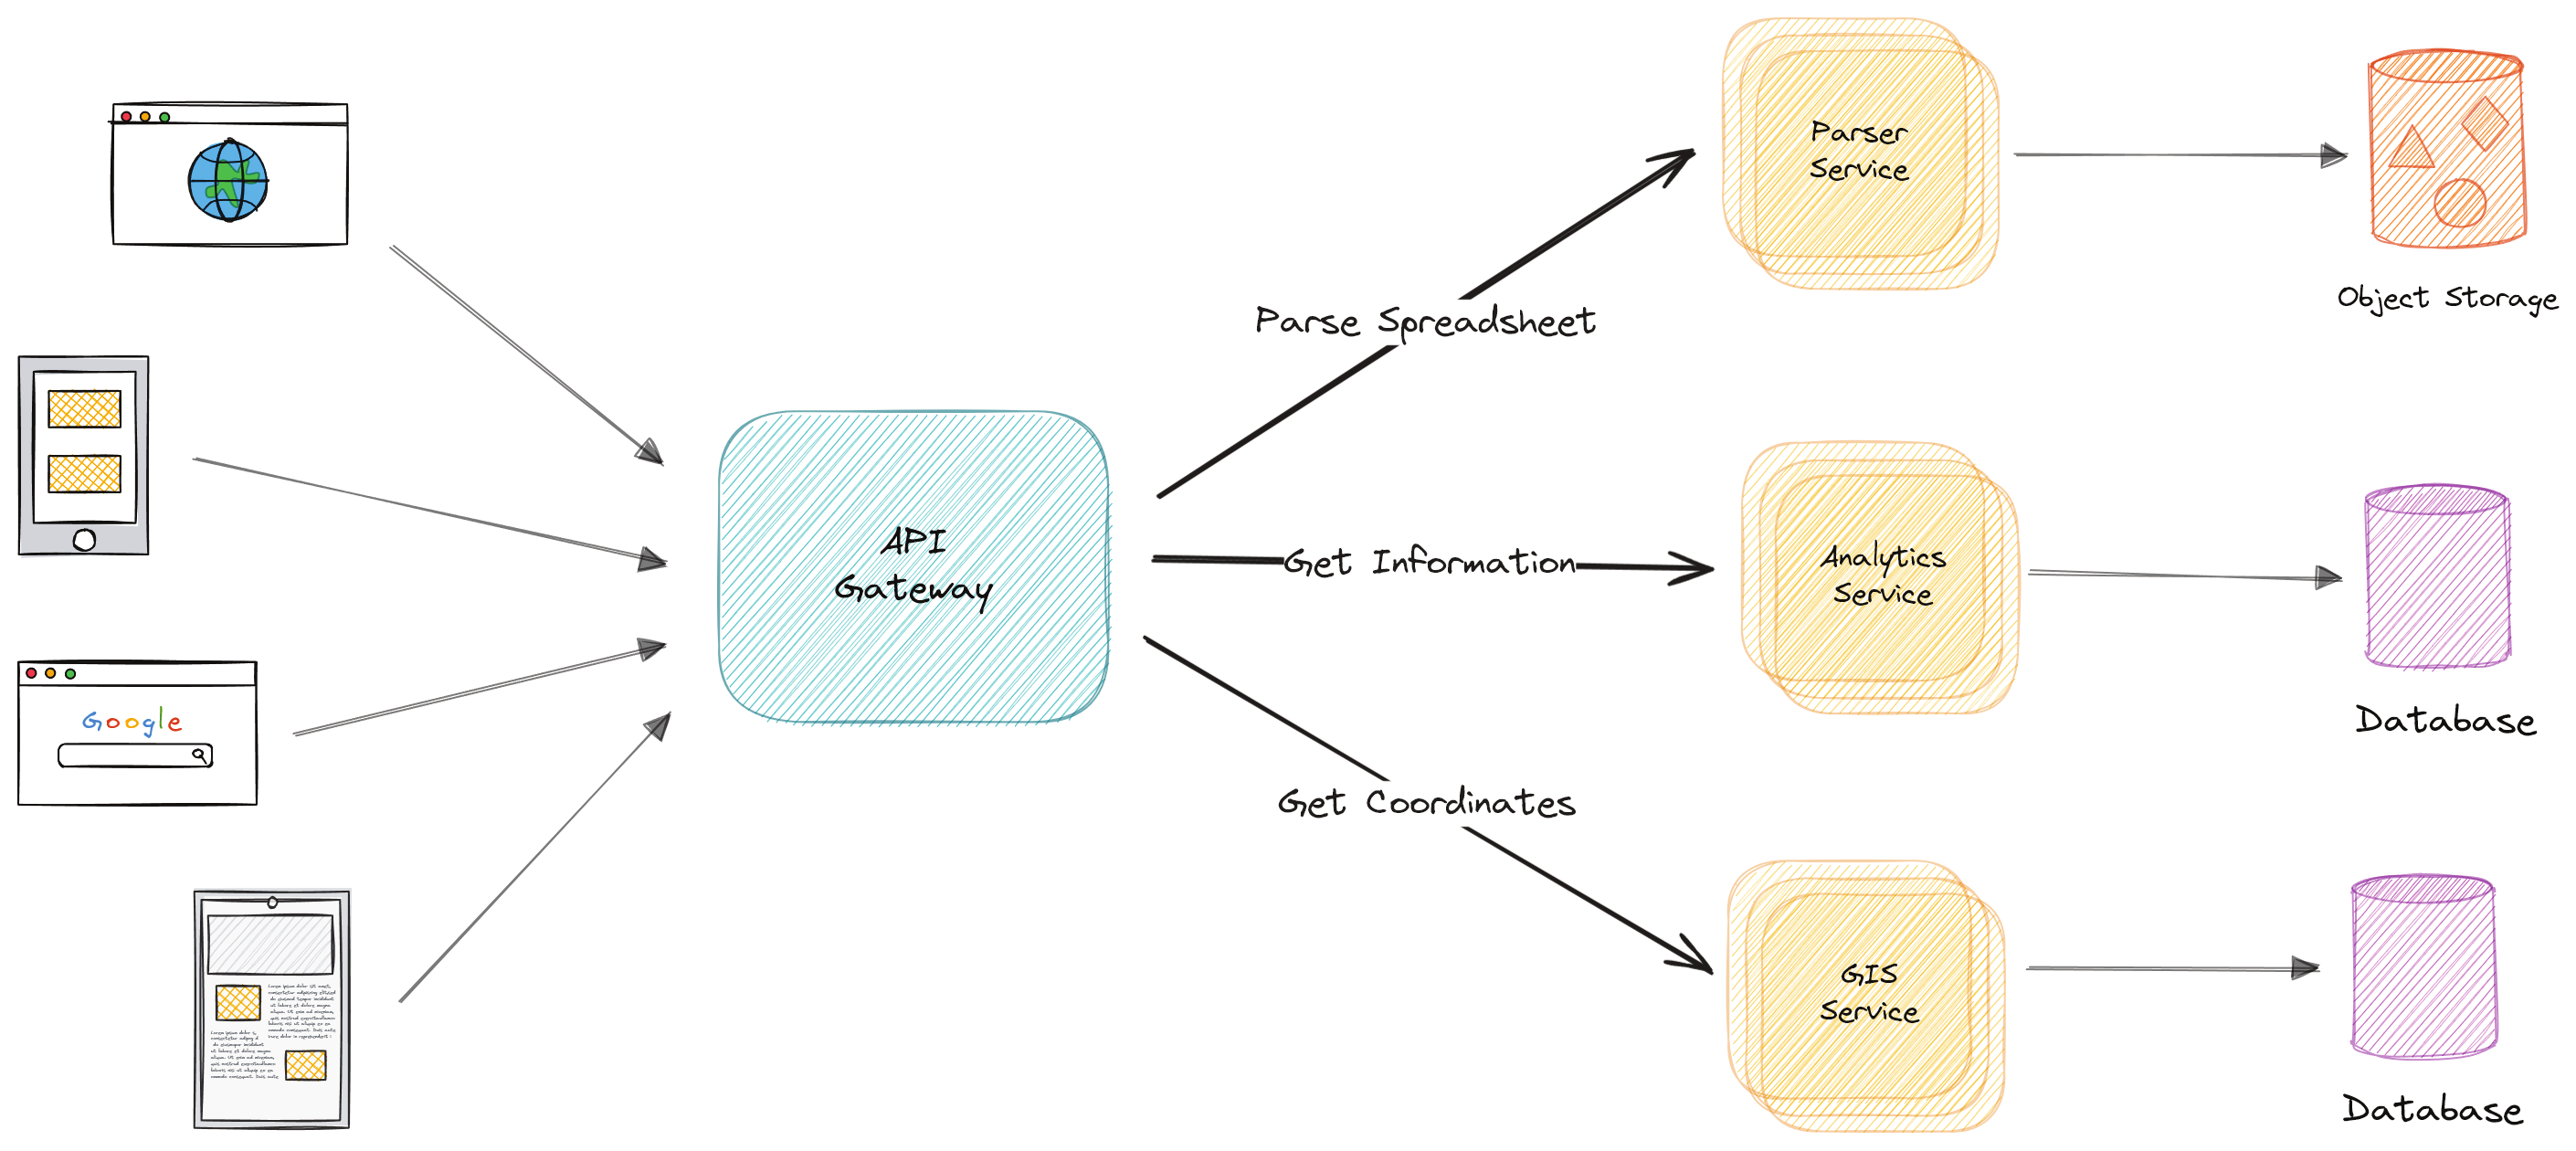
\includegraphics[width=0.7\textwidth]{Dissertation/images/bff_par}
    \caption{Схема параллельной обработки запросов в BFF}
    \label{fig:bff_parallel_processing}
\end{figure}

\paragraph{Сравнительный анализ решений API Gateway}

Сравнительный анализ решений API Gateway основывается на критериях производительности, масштабируемости, безопасности, интеграции, удобства использования и поддержки сообщества. Анализ включает Spring Cloud Gateway, Kong, Amazon API Gateway, Apigee и NGINX.

Spring Cloud Gateway демонстрирует высокую производительность благодаря реактивной архитектуре на основе Spring WebFlux, обеспечивающей асинхронную обработку и высокую пропускную способность.
Kong характеризуется аналогичной производительностью благодаря использованию NGINX и LuaJIT. Spring Cloud Gateway легко масштабируется в экосистеме Spring Cloud с поддержкой кластеризации и интеграции с системами оркестрации~\cite{carnell2021spring}. Kong поддерживает горизонтальное масштабирование и интеграцию с контейнерными оркестраторами.

Spring Cloud Gateway поддерживает интеграцию с решениями аутентификации и авторизации, включая OAuth2 и JWT. Kong обладает комплексными функциями безопасности, включающими SSL/TLS шифрование и контроль доступа на уровне API.

Spring Cloud Gateway, благодаря высокой производительности, простоте интеграции с экосистемой Spring и обширному сообществу, является оптимальным выбором для проектов на базе Spring. Решение обеспечивает необходимую гибкость, масштабируемость и безопасность для современных микросервисных архитектур.


Для платформы аналитики исторических данных API Gateway должен обеспечивать маршрутизацию запросов в различные версии сервисов, поддержку OAuth 2.0 для передачи информации о пользователе, сбор метрик и логирование.
Spring Cloud Gateway полностью соответствует данным требованиям~\cite{spring_cloud_gateway}. Ключевым преимуществом является работа в неблокирующем режиме.

Неблокирующая архитектура, реализованная на основе Netty и проекта Reactor, представляет собой асинхронный фреймворк с циклами событий. Архитектура может использовать минимальное количество потоков, где каждый процессорный поток управляет циклом событий с каналами для обработки входящих соединений.

Запрос поступает через HTTP в канал, обрабатывается циклом событий и передается в приложение WebFlux как объект ServerHttpRequest. Обработка происходит в неблокирующем режиме: цикл событий создает флаг ожидания ответа и готов принимать новые запросы.
WebFlux оборачивает запрос в ServerWebExchange и передает его через цепочку обработчиков до WebClient.

В процессе взаимодействия микросервисов при синхронных вызовах существует вероятность недоступности или высокой задержки~\cite{richardson_circuit_breaker}. Это может привести к блокировке ресурсов вызывающей стороны и неспособности обработки других запросов.

Для обеспечения надежного взаимодействия используется прокси-сервер, функционирующий по принципу электрического выключателя~\cite{richardson2018microservices}. При достижении порога последовательных сбоев происходит автоматическое срабатывание, и в течение периода ожидания все попытки обращения завершаются неудачей.
После истечения времени ожидания пропускается ограниченное количество тестовых запросов.

API-шлюз использует паттерн Circuit Breaker, реализованный через Spring Cloud Circuit Breaker и Resilience4j.

\subsection{Проектирование безопасности}

Обеспечение максимальной безопасности и конфиденциальности данных пользователей является приоритетной задачей проекта.
Реализован отдельный авторизационный сервис, функционирующий по протоколам OAuth2.0 и OpenID~\cite{18_hardt2012,openid_foundation2014}.

OAuth2 представляет собой протокол авторизации для безопасной передачи данных между сторонними сервисами~\cite{richer2017}.
Протокол позволяет пользователям предоставлять доступ к данным без передачи паролей. Приложение получает токен доступа от сервера авторизации для последующего доступа к ресурсам пользователя~\cite{18_hardt2012}.
Важные аспекты безопасности OAuth2.0 детально рассмотрены в специальной спецификации угроз и мер безопасности~\cite{lodderstedt2013}, а формальный анализ безопасности протокола представлен в работе~\cite{fett2016}.

OpenID представляет открытый стандарт децентрализованной системы аутентификации, позволяющий создать единую учетную запись для множества интернет-ресурсов через услуги третьих лиц~\cite{19_weingartner2017,sakimura2015}.
OpenID Connect функционирует как идентификационный слой поверх OAuth 2.0, обеспечивая надежную аутентификацию пользователей~\cite{openid_foundation2014}.

На рисунке~\ref{fig:openid_diagram} можно увидеть диаграмму деятельности OpenID.
\begin{figure}[htbp]
    \centering
    % Placeholder для диаграммы деятельности OpenID
    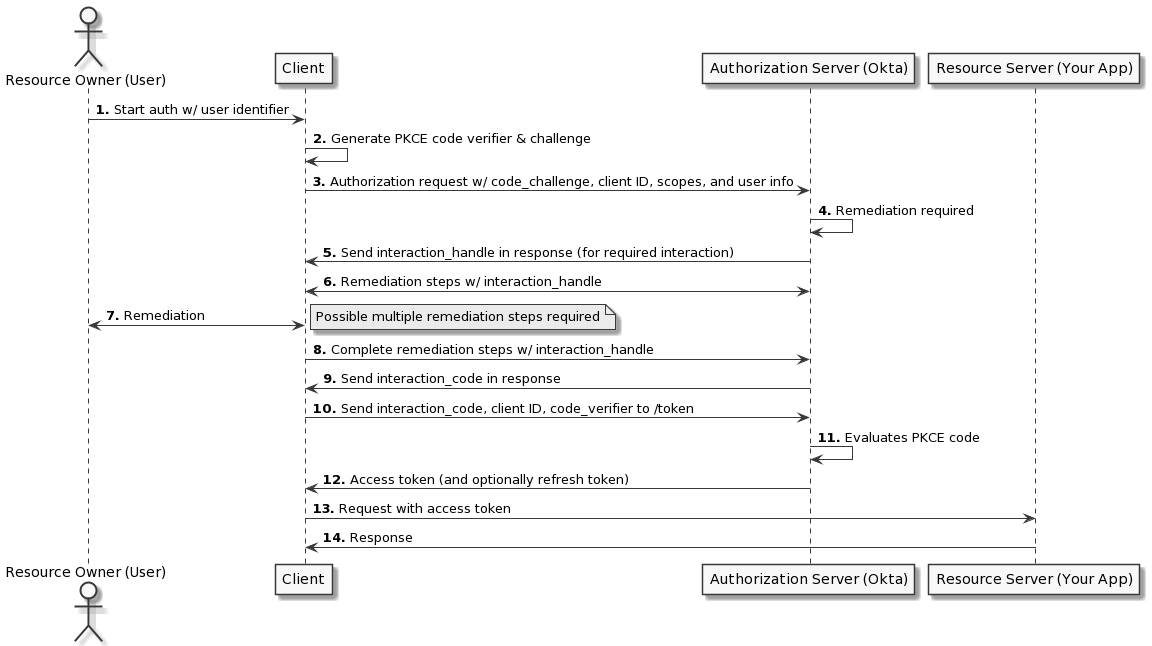
\includegraphics[width=0.7\textwidth]{Dissertation/images/openId_scheme}
    \caption{Диаграмма деятельности OpenID}
    \label{fig:openid_diagram}
\end{figure}

Реализация системы безопасности на основе OpenID и OAuth2 обеспечивает современный уровень защиты данных и соответствует международным стандартам информационной безопасности~\cite{fett2016,19_weingartner2017}.
